%!TEX root = ../PTC-LibUG.tex
\linenumberfrequency{0}

\chapter{Computing Accelerator Properties}
\label{cha:accel.properties}

\index{accelerator!properties}
\index{property!accelerator}
This chapter explains how to compute global and local accelerator
properties and provides examples of the code required for the computations.


\section{Global Scalars}

\index{global property!described}
\index{property!global}
\index{global property|see{\emph{also} global information}}
\index{closed orbit!global properties}
%
Global scalars apply to the accelerator as a whole. They can be
derived only after the complete accelerator has been modeled, and
they are the same at any point on the closed orbit.


\subsection{Tunes}

\makeusother
\begin{ptccode}
x = zero
x(5) = delta
call find_orbit(lattice, x, 1, istate, 1.d-7)
call init(istate, 1, 0)
call alloc(y)
call alloc(normal)
call alloc(id)
id = 1
y = x + id
call track(lattice, y, 1, istate)
normal = y
write(6,'(a,3(2x,f9.6))') 'tunes:', normal%tune
\end{ptccode}
\makeussubscript


\subsection{Chromaticity}

%\makeusother
%\begin{ptccode}
%\end{ptccode}
%\makeussubscript


\subsection{Anharmonicity}

%\makeusother
%\begin{ptccode}
%\end{ptccode}
%\makeussubscript


\section{s-Dependent Global Quantities}

\subsection{Betatron Amplitude}

\makeusother
\begin{ptccode}
x = zero
x(5) = delta
call find_orbit(lattice, x, 1, istate, 1.d-7)
call init(istate, 1, 0)
call alloc(y)
call alloc(normal)
call alloc(id)
id = 1
y = x + id
call track(lattice, y, 1, istate)
normal = y
y = x + normal%a_t  ! track this---normalizing transformation
p => lattice%start
beta_x = (y(1).sub.'10') ** 2   + (y(1).sub.'01') ** 2
beta_y = (y(3).sub.'0010') ** 2 + (y(3).sub.'0001') ** 2
write(6,'(a,2(2x,f9.6))') 'beta_x, beta_y: ', beta_x, beta_y
do j = 1, lattice%n
  call track(lattice, y ,j, j+1, istate)
  beta_x = (y(1).sub.'10') ** 2   + (y(1).sub.'01') ** 2
  beta_y = (y(3).sub.'0010') ** 2 + (y(3).sub.'0001') ** 2
  write(6,'(a,2(2x,f9.6))') 'beta_x, beta_y: ', beta_x, beta_y
  p => p%next
end do
\end{ptccode}
\makeussubscript


%\subsection{Twiss Parameter}

%\makeusother
%\begin{ptccode}
%\end{ptccode}
%\makeussubscript


\subsection{Dispersion}

\makeusother
\begin{ptccode}
x = zero
x(5) = delta
call find_orbit(lattice, x, 1, istate, 1.d-7)
call alloc(id)      ! type(damap)
call alloc(disp)    ! type(damap)
call alloc(xt)      ! type(damap)
call alloc(eta)     ! type(real_8), dimension(6)
call alloc(y)       ! type(real_8), dimension(6)
call alloc(normal)  ! type(normalform)
id = 1
y = x + id
call track(lattice, y, 1, default)
normal = y
y = x + normal%A_t
p => lattice%start
do j = 1, lattice%n
  call track(lattice, y ,j, j+1, default)
  id = 0
  xt = y
  disp = xt * id
  x = xt
  id = 1
  disp = id - disp
  xt = disp * xt
  eta = x + xt
  dispx = (eta(1).sub.'00001')
  dispy = (eta(3).sub.'00001')
  write(6,'(a,2(2x,f9.6))') 'disp_x, disp_y: ', dispx, dispy
end do
\end{ptccode}
\makeussubscript


\subsection{Phase Advance}

\begin{marginfigure}
  \centering
  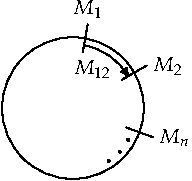
\includegraphics{MetaPost/PhaseAdvance/phaseadv-01}
  \caption{One-turn and partial-turn transfer maps.}
  \label{fig:maps-ring}
\end{marginfigure}

\begin{figure}[htbp]
  \centering
  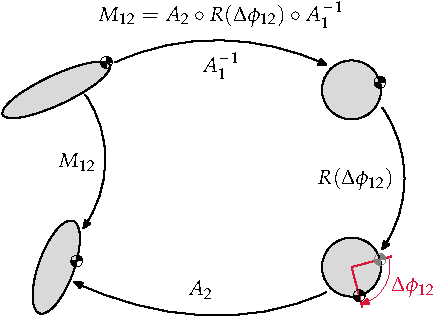
\includegraphics{MetaPost/PhaseAdvance/phaseadv-02}
  \caption{This graphic illustrates the essential relationships between the one-turn map and the normal form at two different locations in a ring lattice.}
  \label{fig:geom-phsadv}
\end{figure}

See caveat at end of \Sref{analyze.accel.prop}!

\makeusother
\begin{ptccode}
x = zero
x(5) = delta
call find_orbit(lattice, x, 1, istate, 1.d-7)
call init(istate, 1, 0)
call alloc(y)
call alloc(normal)
call alloc(id)
id = 1
y = x + id
call track(lattice, y, 1, istate)
normal = y
y = x + normal%a_t
theta_prev = zero
phi = zero
write(6,'(a,2(2x,f9.6))') ' CS phase adv:', phi(1:2)
p => lattice%start
do j = 1, lattice%n
  call track(lattice, y ,j, j+1, istate)
  theta(1) = atan2((y(1).sub.'01'), (y(1).sub.'10')) / twopi
  theta(2) = atan2((y(3).sub.'0001'), (y(3).sub.'0010')) / twopi
  do k = 1, 2
    if(theta(k) < zero .and. abs(theta(k)) > tiny) then
      theta(k) = theta(k) + one
    end if
    dphi(k) = theta(k) - theta_prev(k)
    if(dphi(k) < zero .and. abs(dphi(k)) > tiny) then
      dphi(k) = dphi(k) + one
    end if
    phi(k) = phi(k) + dphi(k)
  end do
  theta_prev = theta
  write(6,'(a,2(2x,f9.6))') ' CS phase adv:', phi(1:2)
  p => p%next
end do
\end{ptccode}
\makeussubscript


\subsection{Beam Envelope}

Text and example code here.
%\makeusother
%\begin{ptccode}
%\end{ptccode}
%\makeussubscript


\section{Local Quantities}

\index{local property!described}
\index{property!local}
\index{local property|see{\emph{also} local information}}
\index{closed orbit!local properties}
%
Local properties do not apply to the accelerator as a whole. They
are derived from individual magnets, and they differ at different
points on the closed orbit. The trajectory of a particle through a
magnet is local; it is derivable from the individual magnet irrespective
of the magnet's position in the accelerator.

\endinput
